\section{Measuring pooling bias}
\label{sec:analysis}
%(1 pages)

% Primer
The example in \figureref{pooling} makes it apparent that pooling-based evaluation can introduce a systematic bias against unpooled systems.
However, it has been assumed that the bias is insignificant in practice given the large number of systems pooled in the TAC KBP evaluation.
We will now show that the assumption is not valid using data from the TAC KBP 2015 evaluation.\footnote{%
Our results are not qualitatively different on data from previous years of the shared task.}

% Data and methodology
\begin{figure}[t]
  \centering
  \begin{subfigure}{\columnwidth}
      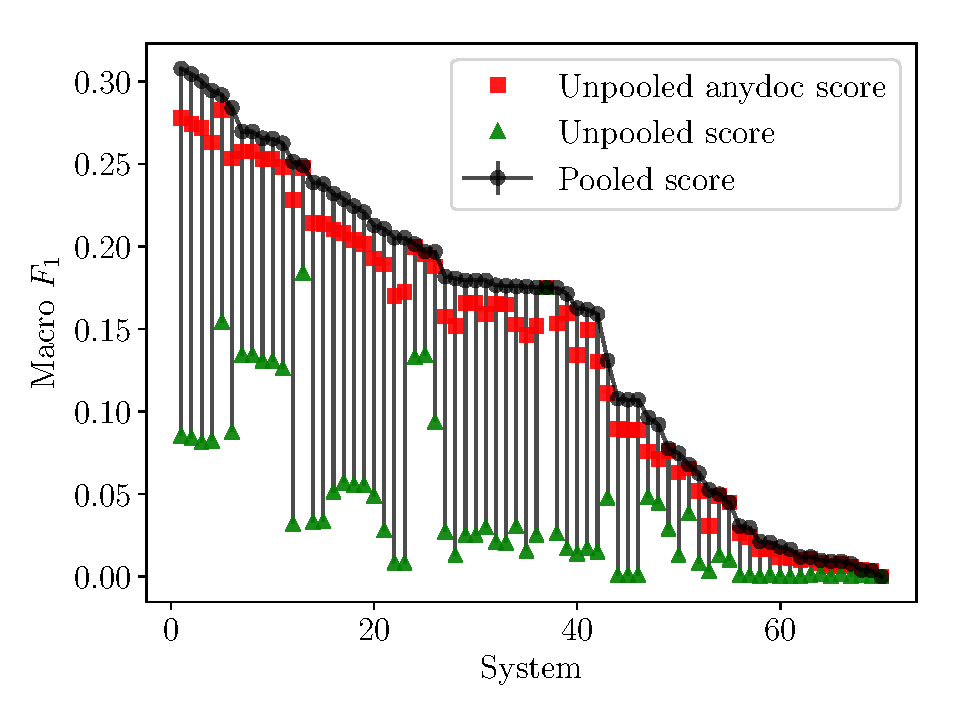
\includegraphics[width=\columnwidth]{figures/pooling_bias/pooling_bias}
    \centering
    \small{\begin{tabular} {l r r r} \toprule
                    & \multicolumn{3}{c}{Median bias} \\
                    & Precision & Recall & Macro \fone{} \\ \midrule 
   Official         & 17.93\% &  17.00\% & 15.51\% \\ 
   \anydoc{}        & 2.34\% &  1.93\% & 2.05\% \\ \bottomrule
   \end{tabular}}
  \end{subfigure}
  \caption{\label{fig:pooling-bias} Median pooling bias on the top 40 systems of TAC KBP 2015 evaluation using the official and \anydoc{} scores.
  The bias, even with the lenient \anydoc{} metric, is larger than the largest difference between adjacent systems (1.5\% \fone{}) and typical system improvements (around 1\% \fone{}),
  invalidating the assumption that pooling bias is insignificant.
  }
\end{figure}
\paragraph{Measuring bias.}
In total, there are 70 system submissions from 18 teams for 317 query entities and the evaluation set consists of 11,008 assessed relation instances.\footnote{%
  The evaluation set is actually constructed from compositional queries like, ``what does Carrie Fisher's parents do?'':
  these queries select relation instances that answer the question ``who are Carrie Fisher's parents?'', and then use those answers (e.g.\ ``Debbie Reynolds'') to select relation instances that answer ``what does Debbie Reynolds do?''.
  We only consider instances selected in the first part of this process.
}
The original evaluation dataset gives us a good measure of the true scores for the participating systems.
Similar to \citet{zobel1998reliable}, which studied pooling bias in information retrieval,
simulate the condition of a team not being part of the pooling process by removing any predictions that are unique to its systems from the evaluation dataset.
The pooling bias is then the difference between the true and unpooled scores.

\paragraph{Results.}
\reffig{pooling-bias} shows the results of measuring pooling bias on the TAC KBP 2015 evaluation on the \fone{} metric using the official and \anydoc{} scores.\footnote{%
  We note that \anydoc{} scores are on average 0.88\%\fone{} larger than the official scores. 
  }\footnote{
  The outlier at rank 36 corresponds to a University of Texas, Austin system that only filtered predictions from other systems and hence has no unique predictions itself.
  }
We observe that even with lenient \anydoc{} heuristic, the median bias (2.05\% \fone{}) is much larger than largest difference between adjacently ranked systems (1.5\% \fone{}).
This experiment shows that pooling evaluation is significantly and systematically biased against systems that make novel predictions!

%  We also considered an alternate scoring model where relation instances outside the evaluation set were of ignored instead of marked wrong and find that under this model \fone{} scores remain biased by 14.99\% and 0.73\% points on average, with and without the \anydoc{} heuristic respectively.
%% TODO:  \ap{elaborate methodology}
%While this scoring model is less biased than assuming unassessed relation instances to be wrong, combined with the discrepancy of the \anydoc{} score it remains too large a difference to be ignored.
%The analysis confirms the necessity of the \anydoc{} heuristic during development evaluations,
%  but at the same time, even with the heuristic, the bias is much larger than the typical system difference.
%Thus, we conclude that this evaluation is biased against improvements that lead to novel predictions!

% OLD as of 4/9/17
% % TODO: Need to state explicitly this is for entity scores.
% 
% The closed-world assumption is well understood to provide pessimistic estimates of system performance \pl{based on what?}, but its bias has not been measured before.
% The prevailing intuition is that the evaluation set probably covers most of the correct relations because only instances pertaining to a very specific set of relations are evaluated.
% %In this section, we will describe what kinds of predictions are falsely marked negative by the closed world heuristic, how the resulting bias can be measured and finally present results regarding the bias in the context of TAC KBP.
% In this section, we will describe how the resulting bias can be measured and discuss results regarding the bias in the context of TAC KBP.\@
% 
% %\paragraph{False negatives.}
% %% What are the different ways that systems predict new facts?
% %Let's assume that our evaluation set contains only the relation instance shown in \figureref{example}, which identifies Debbie Reynolds as a parent of Carrie Fisher.
% %There are few ways that the closed world assumption can falsely predict a relation instance to be wrong.
% %First, the instance may state known information but from a different place, e.g.\ from the sentence 
% %  ``\textit{Carrie Frances Fisher} was born \ldots to actors and singers Eddie Fisher and \textit{Debbie Reynolds}.''
% %% TODO: "object string" is clunky.
% %Secondly, a relation instance may state known information but use a different string for the object, e.g.\ a system might use ``Mary Frances Reynolds'' instead of ``Debbie Reynolds'', which is a nickname.
% %Finally, a relation instance may express an entirely new relation, e.g.\ that ``Eddie Fisher'' is Carrie's father.
% %In all the above cases, the closed world assumption considers the instance to be wrong.
% %With the \anydoc{} heuristic, the first instance is correctly marked, but this heuristic also incorrectly marks the instance, ``Bright Lights: Starring Carrie Fisher and Debbie Reynolds'' as being true.
% %Consequently, 
% %  while the closed world assumption is a strict underestimate of performance, the \anydoc{} heuristic is not guaranteed to be.
% 
% % Remind closed world assumption.
% % How do we measure the effects of CWA on development?
% % Ideally, we would like to measure the performance of development runs and see ifthere are potentially useful contributoins that could have been used had it not been for the evaluation.
% % We can't do that, but we can compare how teams that participated in the evaluation might have fared had they not been part of the evaluation. 
% % To do so, we use the SVT data...
% % For each submission, we compare its scores with the hypothetical scores of how the system would have done the team had not participated in the construction of the evaluation data.
% % describe results
% % describe consequences.
% 
% \pl{think of a simple figure / example to show the bias;
% this is an important point and a simple concept;
% I bet that there's a figure that someone could look at for 5 seconds and understand
% }
% 
% \paragraph{Measuring bias.}
% \begin{figure*}[t]
%   \begin{subfigure}{\columnwidth}
%   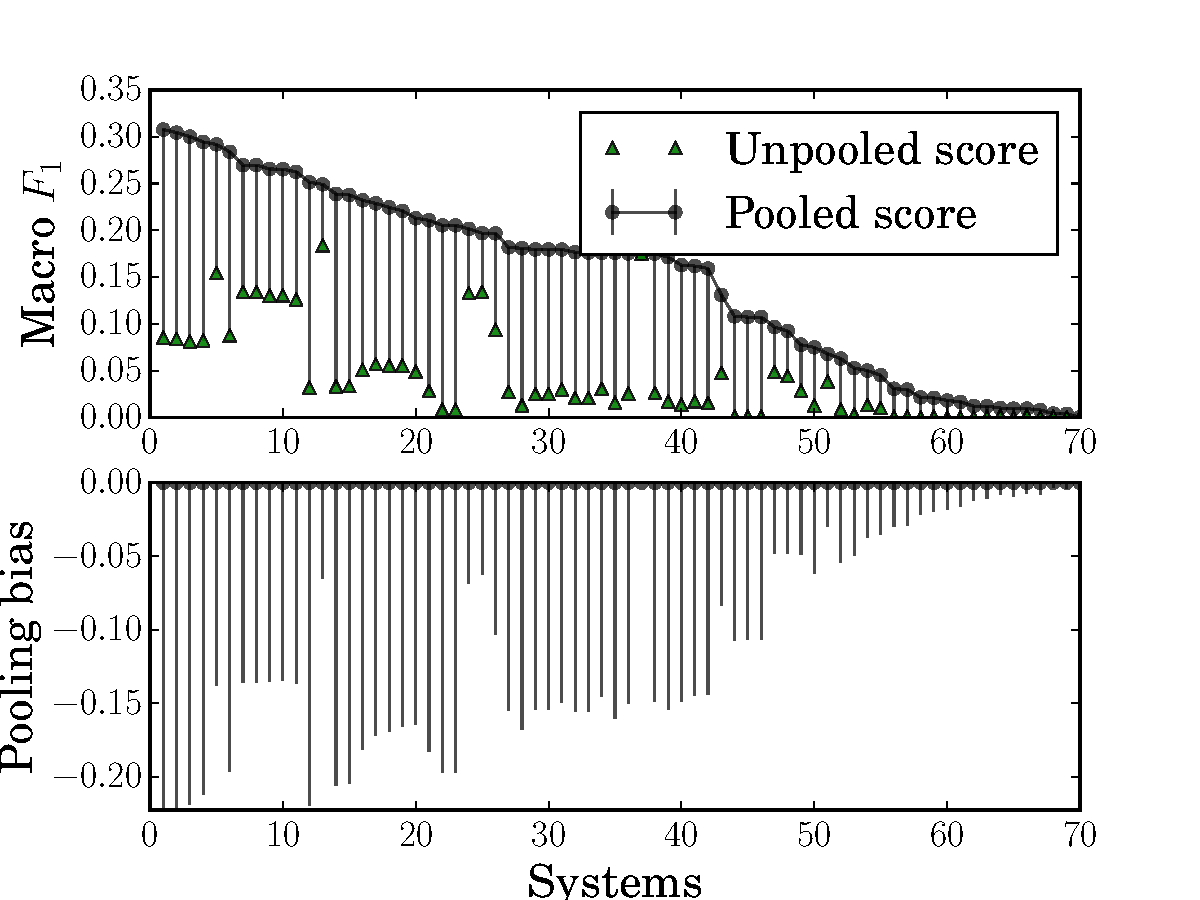
\includegraphics[width=\columnwidth]{figures/pooling_bias/pooling_bias_closed-world}
%   \caption{Pooling bias for macro \fone{} scores without the \anydoc{} heuristic.}
%   \end{subfigure}
%   \begin{subfigure}{\columnwidth}
%   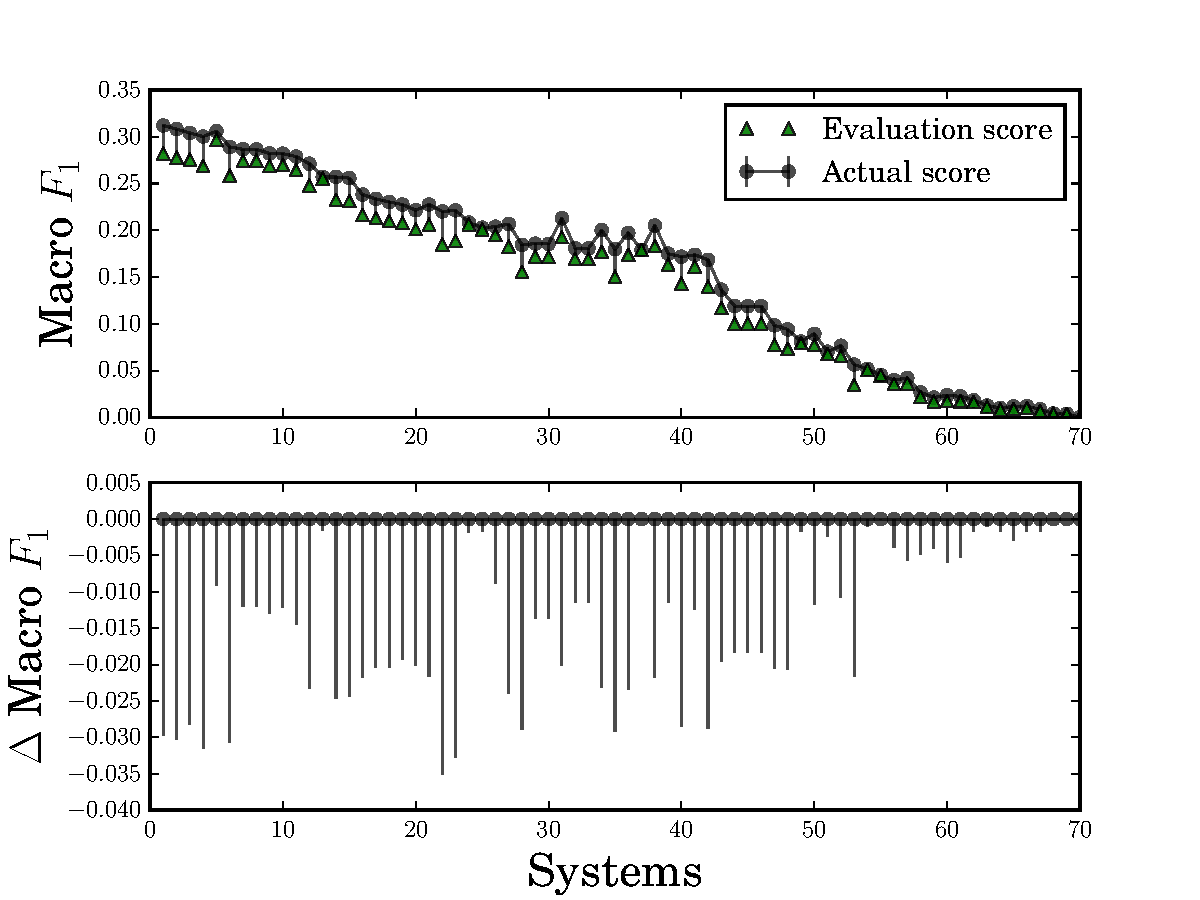
\includegraphics[width=\columnwidth]{figures/pooling_bias/pooling_bias_anydoc}
%   \caption{Pooling bias for macro \fone{} scores with the \anydoc{} heuristic.}
%   \end{subfigure}
%   \caption{\label{fig:pooling-bias} Pooling bias measures how much a system's score is affected by not having its output as part of the pooled evaluation.
%   The median bias on the top 40 teams against an unpooled team is 15.51\% points for the standard macro \fone{} metric and 1.98\% when evaluating using the \anydoc{} heuristic.
%   Note that the median difference between the \anydoc{} scores and standard scores is 0.74\% points; this difference is caused because the \anydoc{} heuristic erroneously scores fills with incorrect judgements to be correct.}
% \end{figure*}
% 
% Ideally, we would like to measure the difference between performance scores of development systems on the evaluation set and a hypothetical set that includes evaluations of all its relations.
% This difference is often called the ``pooling bias'' in information retrieval literature~\citep{}. % TODO: cite weber and many others.
% As a proxy to development systems, we will make use of system submissions to the TAC KBP 2015 competition, made available through the TAC KBP Slot Validation Tracks~\citep{}.
% There are 70 submissions from 18 teams for 317 queries and the evaluation set consists of 11,008 assessed relation instances.\footnote{%
%   The evaluation set is actually constructed from compositional queries like, ``what does Carrie Fisher's parents do?'':
%   these queries select relation instances that answer the question ``who are Carrie Fisher's parents?'', and then use those answers (e.g.\ ``Debbie Reynolds'') to select relation instances that answer ``what does Debbie Reynolds do?''.
%   We only consider instances selected in the first part of this process.
% }
% Adopting the methodology of \citet{weber2010measurement},
% we construct a hypothetical evaluation set for each submission to simulate what the evaluation set would look like if the corresponding team did not submit its results.
% This hypothetical evaluation set contains only those relations that were predicted by at least one other system or the human annotators.
% We then measure the difference between performance scores on the original evaluation set and on the hypothetical evaluation set with and without the \anydoc{} heuristic. 
% 
% \paragraph{Results.}
% \figureref{pooling-bias} summarizes our results on pooling bias for the macro \fone{} metric.
% The effect of bias is truncated on systems that performed very poorly.
% Consequently, we report median results on the top 40 systems (which corresponding to a sharp drop in performance).
% The outlier in the graph at rank 36 corresponds to a submission from University of Texas, Austin that only filtered outputs from other systems: this submission does not suffer any pooling bias because all of its outputs are included in the hypothetical evaluation set.
% 
% Without the \anydoc{} heuristic, pooling bias is 15.51\% \fone{} points and with the heuristic it is 1.98\% \fone{} points.
% We note that the \anydoc{} heuristic overestimates scores by about 0.74\% \fone{} points.
% The bias affects precision and recall almost equally: 
%   the median bias the without \anydoc{} heuristic being 17.93\% and 17.0\% respectively, and
%   the median bias the with \anydoc{} heuristic being 2.34\% and 1.93\% respectively.
% We also consider the alternate heuristic of ignoring relation instances outside the evaluation set and find that that biases \fone{} scores upwards by \fake{3\%}.
% At the same time, the median difference between two adjacent submissions is only 0.3\%\fone{} with largest difference being 1.5\% \fone{} (between the 26th and 27th ranked submissions).
% This analysis confirms the necessity of the \anydoc{} heuristic during development evaluations,
%   but at the same time, even with the heuristic, the bias is much larger than the typical system difference.
% Thus, we conclude that this evaluation is biased against novel system improvements!
% 
% %  the median bias against an unpooled team is 13.55\% \fone{} points and for an unpooled system is 4.55\% \fone{} points,
% %  making it impossible to evaluate against this metric in development (also significantly biasing new entrants to the task).
% %The former is a proxy that measures how much bias development systems of teams that had participated in the KBP evaluation experience and the latter measures the bias development systems of new teams experience.
% %\figureref{pooling-bias} shows the pooling bias experienced by teams and systems in the 2015 evaluation;
% %  the median bias against an unpooled team is 13.55\% \fone{} points and for an unpooled system is 4.55\% \fone{} points,
% %  making it impossible to evaluate against this metric in development (also significantly biasing new entrants to the task).
% %
% 
% % We will make use of system submissions released as part of the TAC KBP Slot Validation tracks in 2013, 2014 and 2015.
% % The 2015 dataset contains 70 submissions from 18 teams for 317 queries.
% % Considering only the submissions to the first hop of the two-hop \pl{to non-KBP person, don't know what this means} evaluation,
% % each submission contains on average about 35,951 predicted slotfills. 
% % There are in total 201,332 relations that were predicted, of which only 11,008 of these slotfills have were evaluated.
% 
% %  each submission predicts on average
% %We will make use of system submissions released as part of the TAC KBP Slot Validation tracks in 2013, 2014 and 2015.
% %The 2015 dataset contains 70 submissions from 18 teams for 317 queries.
% %Considering only the submissions to the first hop of the two-hop \pl{to non-KBP person, don't know what this means} evaluation,
% %each submission contains on average about 35,951 predicted slotfills. 
% %There are in total 201,332 relations that were predicted, of which only 11,008 of these slotfills have were evaluated.
% %
% %The ``gold'' labels on relation contexts are collected by a combination of a time-bounded human search in the corpus and a human evaluation of pooled output from participating systems.
% %While the human search identifies a significant fraction of relations (\todo{80\%}),
% %  it does not sufficiently cover the variety of contexts that are submitted as justifications of the relation. 
% %This has two implications on how a development system, \textit{D}, that did not participate in the original evaluation is scored.
% %Firstly, it is likely that contexts \pl{I thought the problem with bias was due to the set of relations $D$ returns, not contexts} the system \textit{D} submits has never been seen before and hence can not be evaluated.
% %Secondly, it is also likely that relations the system \textit{D} submits have never been seen before, particularly if \textit{D} incorporates a novel method of relation extraction, creating a perverse incentive to ensure that new extraction methods behave similarly to old extraction systems.
% %The magnitude of this effect, the pooling bias, is can be quantified by performing a ``leave-one-out'' (``leave-team-out'') experiment on previous years submissions, measuring the difference in metric scores when output unique to a single submission (team) is excluded from the gold data.
% %The former is a proxy that measures how much bias development systems of teams that had participated in the KBP evaluation experience and the latter measures the bias development systems of new teams experience.
% %\figureref{pooling-bias} shows the pooling bias experienced by teams and systems in the 2015 evaluation;
% %  the median bias against an unpooled team is 13.55\% \fone{} points and for an unpooled system is 4.55\% \fone{} points,
% %  making it impossible to evaluate against this metric in development (also significantly biasing new entrants to the task).
% %
% %To mitigate this unreasonable bias, teams typically adopt an `anydoc' heuristic during evaluation, which ignores the justification of a context while evaluating a relation.
% %\pl{hard for me to get intuition for implications of anydoc}
% %With this heuristic (\figureref{pooling-bias-anydoc}), the pooling bias decreases considerably, with 
% %  the median bias against an unpooled team being 1.98\% \fone{} points and unpooled system is 0.0\% \fone{} points.
% %However, it should also be noted that scores under the `anydoc' heuristics are on average 0.74\% higher than the standard scores due to erroneously labeling entries to be correct.
% %This analysis confirms the necessity of the `anydoc' heuristic on the current evaluations, but regardless, the bias is large enough to wash out the effect of the typical improvement a development makes.
% % TAKEAWAY: new entrants are biased against!
% 
% % In the latter sections of this paper, we eliminate the problem of pooling evaluation all together by proposing an online evaluation methodology where every new submission is considered and selectively evaluated to ensure statistical validity.
% 
% % \paragraph{Evaluating performance across years.}
% % \fake{This analysis is incomplete, so omitting for your convenience!}
% % % NOTE: should we describe any more statistics?
% % \paragraph{How informative is \fone{} as a metric?}
% % \ac{Ignore for now!}
% % \begin{figure*}
% %   \begin{subfigure}{0.49\textwidth}
% %   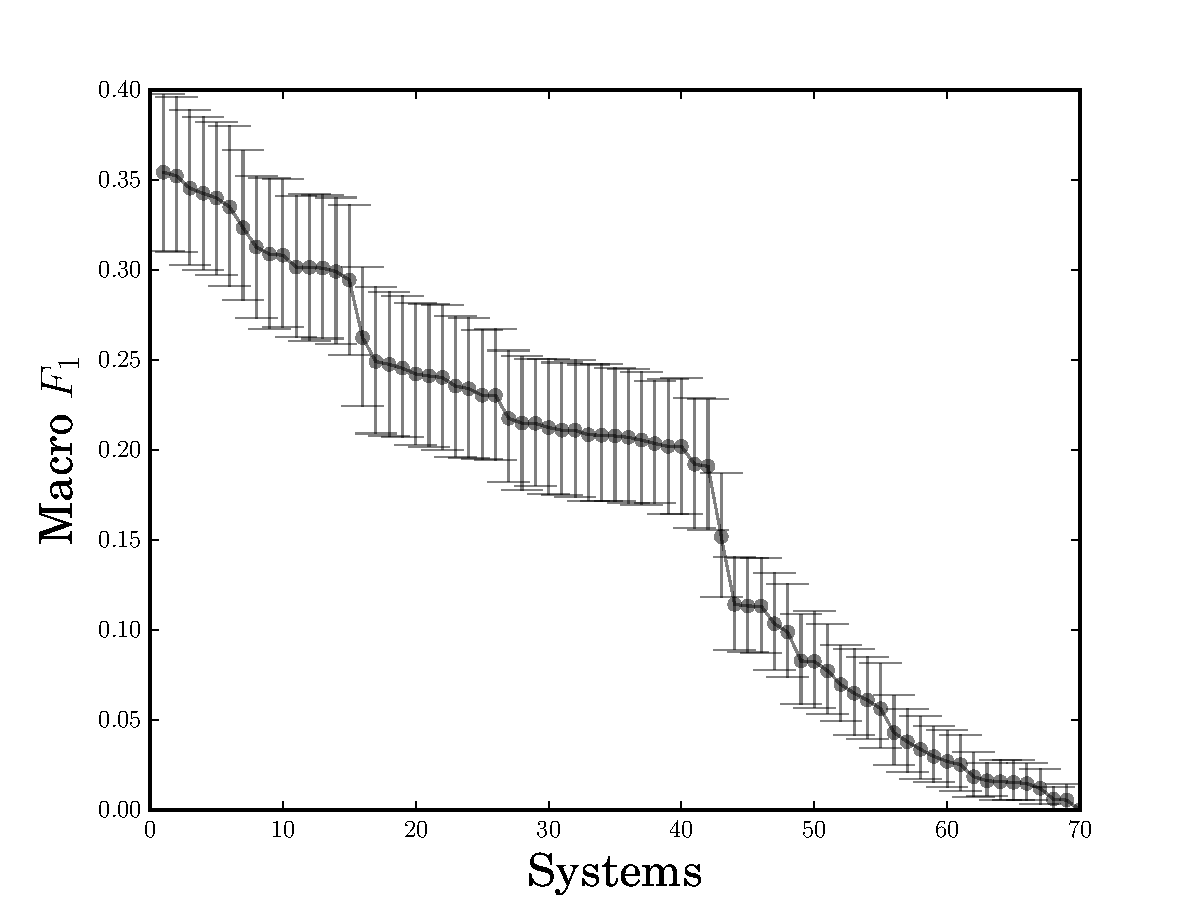
\includegraphics[width=\columnwidth]{figures/experiment1}
% %   \caption{\label{fig:f1}}
% %   \end{subfigure}
% %   \begin{subfigure}{0.49\textwidth}
% %   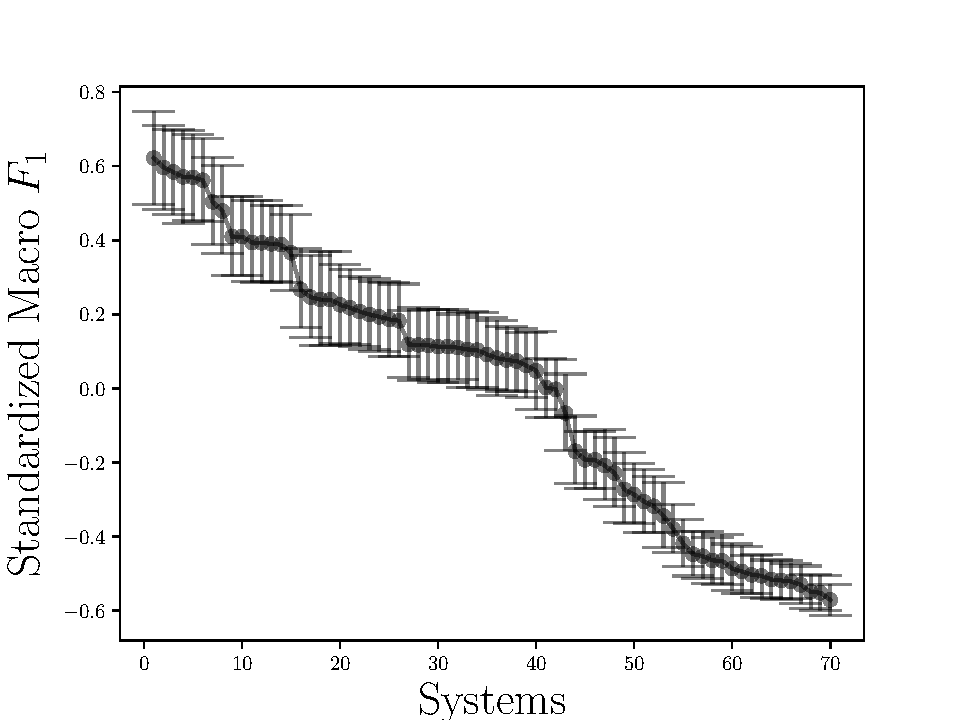
\includegraphics[width=\columnwidth]{figures/experiment3}
% %   \caption{\label{fig:sf1}}
% %   \end{subfigure}
% %   \caption{}
% % \end{figure*}
% % 
% % \begin{table*}
% %   \begin{tabular} {l r r r r r} \toprule
% %     Metric & \multicolumn{3}{c}{Normal} & \multicolumn{2}{c}{Standardized} \\
% %            & Average value & 95\% confidence interval & Mean difference between top 10 teams &  Average value & 95\% confidence interval  \\  \midrule 
% % Micro $P^e$     & $30.91\%$ &  $16.77\%$ & 0.12\% &     &  \\
% % Micro $R^e$     & $30.45\%$ &  $ 6.41\%$ & 0.17\% &     &  \\
% % Micro $\fone^e$ & $38.62\%$ &  $ 6.79\%$ & 0.24\% &     &  \\
% % Macro $P^e$     & $24.98\%$ &  $ 6.93\%$ & 0.24\% &     &  \\
% % Macro $R^e$     & $03.56\%$ &  $ 6.87\%$ & 0.23\% &     &  \\
% % Macro $\fone^e$ & $22.72\%$ &  $ 6.19\%$ & 1.04\% &     &  \\ \bottomrule
% %   \end{tabular}
% % 
% % \begin{tabular}{l r r r r r} \toprule
% %   Metric ($\sigma^2$) & System variance ($\sigma^2_{s}) $ & Query variance($\sigma_{e}$) & Residual ($\sigma_{s,e})$ \\ \midrule % & $\psi$  & $\rho$ \\
% %   \fone{} (0.102) & 11.75\% & 20.59\% & 66.66\% \\ \bottomrule % &     0.120 & 0.152
% % \end{tabular}
% %   \caption{\label{metric-variance}}
% % \end{table*}
% % 
% % Most teams hill climb on a combination of micro and macro entity-level $\fone$ during development.
% % It is natural to ask how much of an improvement on the metric score is necessary to actually trust that system performance has improved.
% % We use a bootstrap sampling \pl{what exactly is being resampled?} method to estimate the variance of $\fone$ and other metrics over query sets \tableref{metric-variance} and measure the 95\% confidence intervals for system scores \figureref{f1}.
% % The median difference in metric scores between adjacent submissions in the top 10 scores (for that metric) is between 0.1--1\%,
% % while the confidence intervals are at least 6\%.
% % % TODO: we can use the differences between the submissions of the each team.
% % It is hard for the researcher to identify if any of the presumably distinct submissions hold any water of another. \pl{awkward}
% % 
% % Next, we would like to ask what factors contribute to the large variance in the system metrics above.
% % One natural confounding variable is the substantial variability in the difficulty of query entities.
% % We can measure the effect of the query entity by analyzing the variation in topic-model scores.
% % Consider the linear model, \pl{$\mu$'s don't cancel out}
% % \begin{align*}
% %   X_{s,e} &= \mu 
% %     + \underbrace{\mu_{s} - \mu}_{\nu_{s}}
% %     + \underbrace{\mu_{e} - \mu}_{\nu_{e}}
% %     + \underbrace{X_{s,e} - \nu_{s} - \nu_{e} - \mu}_{\nu_{s,e}},
% % \end{align*}
% % where $\nu_{s}$, $\nu_{e}$ and $\nu_{s,e}$ capture the effect of the system $s$ and query entity $e$, and the residual.
% % Variance can also be decomposed as,
% % \begin{align*}
% %   \sigma^2(X_{s,e}) &= \sigma^2(\nu_s) + \sigma^2(\nu_e) + \sigma^2(\nu_{s,e}).
% % \end{align*}
% % 
% % \tableref{} shows the variance explained by different components for macro metrics. As we can see, almost twice as much of the variance is explained by the entity only as that of the system.
% % \pl{this is true of any task in general, right, not just KBP?  easy examples everyone gets,
% % hard examples, some people get?}
% % % Explain what the high q,e scores mean.
% % %Another consequence is in confidence intervals.
% % %Bad differentiation from pairwise scores.
% % 
% % % TODO: replace with a GLMM
% % 
% % \paragraph{Controlling for query variance.}
% % \ac{Ignore for now!}
% % 
% % It's easy for us to control for query variance by standardizing our metric,  
% % $$X'_{se} = \frac{X_{se} - \mu_e}{\sigma_e}$$.
% % 
% % \figureref{sf1} plots the performance of systems under the standardized macro \fone metric.
% % % TODO: variance under standardized metric -- showing less contribution
% % % due to queries and an overall reduction in variance.
% % % NOTE: This is only useful when comparing systems, as one is wont to do during development.
% % 
% % % TODO: I wish we could give scroes for this.
% % % \subsection{Are we improving over time?}
% % 
